\section{Partition Coloring Problem}




%Generalization of Network Design Problems
%Several Network Design Problems can be generalized by partitioning the node set V into
%clusters Vk , k ∈ K [5]. Even if those clusters are not necessarily disjunct, the proposed
%algorithms in this thesis requires node disjunct clusters (i. e. Vi ∩ Vj = ∅, ∀i, j ∈ K, i = j).
%A common distinction between three different types (exactly, at least, at most) of such
%generalizations can be done with respect to the number of nodes that need to be in a feasible
%solution of the problem.
%A feasible solution of an exactly generalized problem selects exactly one vertex from each
%cluster Vk (∀k = 1, . . . , r). Similar to that, the at least version requires the solution to
%contain at least one node from each cluster and the at most version requires the solution to
%contain at most one node from each cluster.
%Typically the prefixes E-, L-, and M- are used to distinguish between the different
%generalization types of the same problem (i. e. L-GMST stands for the at least version,
%E-GMST for the exact version, and M-GMST for the at most version of the GMST problem).
%A missing prefix usually refers to the exact generalization of the network design problem.
%This notation will be used in this thesis too as only exact generalizations are considered.

Let $G = (V, E)$ be a non-directed graph and $V$ partitioned into $q$ subsets $V_1, V_2,\ldots, V_q$, where $V_i \cap V_j = \emptyset, \forall i, j = 1, \ldots , q$, $i \neq j$. We refer to $V_1, V_2, \ldots , V_q$ as the components of the partition. The PCP consists in finding a subset $V' \subset V$ such that $|V' \cap V_i| = 1, \forall i = 1, \ldots , q$ (i.e., $V'$ contains one node of each component $V_i$), and the chromatic number of the graph induced in $G$ by $V'$ is minimum.\\
Figure \ref{pd:pcpExample} shows an example of an instance with $10$ nodes and a density of about $0.2$, where density is defined as the probability for each pair of nodes being connected by an edge.

\begin{figure}
\begin{center}
\includegraphics[scale=0.3]{figures/pcp.png}
\caption{(a) Shows a problem instance and (b) its solution.}
\label{pd:pcpExample}
\end{center}
\end{figure}


\section{Wavelength Routing and Assignment Problem}

The PCP has initially been considered by Li and Simha in \cite{li-00} and arises from considering the join problem of routing and wavelength assignment in WDM (Wavelength Division Multiplexing) optical networks. 

%The RWA problem takes two forms: static and dynamic
%[1]. In the static case, all connection requests are known in
%advance, thus a routing decision can be made based on the
%complete knowledge of the traffic to be served by the
%network. The static RWA problem is found to be NP-
%complete that cannot be solved exactly in a polynomial
%T
%This paper resulted from the research supported by the Serbian
%Ministry of science and technological development (project TR-11013).
%Goran Z. Marković is with the Faculty of Traffic and Transport
%Engineering, University of Belgrade, Serbia, Vojvode Stepe 305, 11000
%Belgrade, Serbia; (e-mail:g.markovic@sf.bg.ac.rs).
%Vladanka S. Aćimović-Raspopović is with the Faculty of Traffic and
%Transport Engineering, University of Belgrade, Serbia, Vojvode Stepe
%305, 11000 Beograd, Serbia; (e-mail:v.acimovic@sf.bg.ac.rs).
%time. In the dynamic case, a connection request has to be
%routed and wavelengths assigned independently of other
%connections, which either have already been assigned or
%will be assigned [1]-[3]

\subsection{Example}

\begin{center}
\begin{figure}
\centering
\ifx\du\undefined
  \newlength{\du}
\fi
\setlength{\du}{15\unitlength}


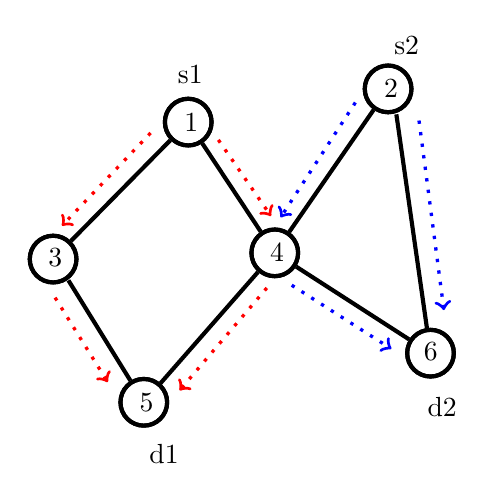
\begin{tikzpicture}
\pgftransformxscale{1.000000}
\pgftransformyscale{-1.000000}
\definecolor{dialinecolor}{rgb}{0.000000, 0.000000, 0.000000}
\pgfsetstrokecolor{dialinecolor}
\definecolor{dialinecolor}{rgb}{1.000000, 1.000000, 1.000000}
\pgfsetfillcolor{dialinecolor}
\pgfsetlinewidth{0.100000\du}
\pgfsetdash{}{0pt}
\pgfsetdash{}{0pt}
\pgfsetbuttcap
\pgfsetmiterjoin
\pgfsetlinewidth{0.100000\du}
\pgfsetbuttcap
\pgfsetmiterjoin
\pgfsetdash{}{0pt}
\definecolor{dialinecolor}{rgb}{1.000000, 1.000000, 1.000000}
\pgfsetfillcolor{dialinecolor}
\pgfpathellipse{\pgfpoint{14.562500\du}{15.212500\du}}{\pgfpoint{0.562500\du}{0\du}}{\pgfpoint{0\du}{0.562500\du}}
\pgfusepath{fill}
\definecolor{dialinecolor}{rgb}{0.000000, 0.000000, 0.000000}
\pgfsetstrokecolor{dialinecolor}
\pgfpathellipse{\pgfpoint{14.562500\du}{15.212500\du}}{\pgfpoint{0.562500\du}{0\du}}{\pgfpoint{0\du}{0.562500\du}}
\pgfusepath{stroke}
\pgfsetbuttcap
\pgfsetmiterjoin
\pgfsetdash{}{0pt}
\definecolor{dialinecolor}{rgb}{0.000000, 0.000000, 0.000000}
\pgfsetstrokecolor{dialinecolor}
\pgfpathellipse{\pgfpoint{14.562500\du}{15.212500\du}}{\pgfpoint{0.562500\du}{0\du}}{\pgfpoint{0\du}{0.562500\du}}
\pgfusepath{stroke}
\pgfsetlinewidth{0.100000\du}
\pgfsetdash{}{0pt}
\pgfsetdash{}{0pt}
\pgfsetbuttcap
\pgfsetmiterjoin
\pgfsetlinewidth{0.100000\du}
\pgfsetbuttcap
\pgfsetmiterjoin
\pgfsetdash{}{0pt}
\definecolor{dialinecolor}{rgb}{1.000000, 1.000000, 1.000000}
\pgfsetfillcolor{dialinecolor}
\pgfpathellipse{\pgfpoint{16.747500\du}{18.662500\du}}{\pgfpoint{0.562500\du}{0\du}}{\pgfpoint{0\du}{0.562500\du}}
\pgfusepath{fill}
\definecolor{dialinecolor}{rgb}{0.000000, 0.000000, 0.000000}
\pgfsetstrokecolor{dialinecolor}
\pgfpathellipse{\pgfpoint{16.747500\du}{18.662500\du}}{\pgfpoint{0.562500\du}{0\du}}{\pgfpoint{0\du}{0.562500\du}}
\pgfusepath{stroke}
\pgfsetbuttcap
\pgfsetmiterjoin
\pgfsetdash{}{0pt}
\definecolor{dialinecolor}{rgb}{0.000000, 0.000000, 0.000000}
\pgfsetstrokecolor{dialinecolor}
\pgfpathellipse{\pgfpoint{16.747500\du}{18.662500\du}}{\pgfpoint{0.562500\du}{0\du}}{\pgfpoint{0\du}{0.562500\du}}
\pgfusepath{stroke}
\pgfsetlinewidth{0.100000\du}
\pgfsetdash{}{0pt}
\pgfsetdash{}{0pt}
\pgfsetbuttcap
\pgfsetmiterjoin
\pgfsetlinewidth{0.100000\du}
\pgfsetbuttcap
\pgfsetmiterjoin
\pgfsetdash{}{0pt}
\definecolor{dialinecolor}{rgb}{1.000000, 1.000000, 1.000000}
\pgfsetfillcolor{dialinecolor}
\pgfpathellipse{\pgfpoint{22.632500\du}{11.112500\du}}{\pgfpoint{0.562500\du}{0\du}}{\pgfpoint{0\du}{0.562500\du}}
\pgfusepath{fill}
\definecolor{dialinecolor}{rgb}{0.000000, 0.000000, 0.000000}
\pgfsetstrokecolor{dialinecolor}
\pgfpathellipse{\pgfpoint{22.632500\du}{11.112500\du}}{\pgfpoint{0.562500\du}{0\du}}{\pgfpoint{0\du}{0.562500\du}}
\pgfusepath{stroke}
\pgfsetbuttcap
\pgfsetmiterjoin
\pgfsetdash{}{0pt}
\definecolor{dialinecolor}{rgb}{0.000000, 0.000000, 0.000000}
\pgfsetstrokecolor{dialinecolor}
\pgfpathellipse{\pgfpoint{22.632500\du}{11.112500\du}}{\pgfpoint{0.562500\du}{0\du}}{\pgfpoint{0\du}{0.562500\du}}
\pgfusepath{stroke}
\pgfsetlinewidth{0.100000\du}
\pgfsetdash{}{0pt}
\pgfsetdash{}{0pt}
\pgfsetbuttcap
\pgfsetmiterjoin
\pgfsetlinewidth{0.100000\du}
\pgfsetbuttcap
\pgfsetmiterjoin
\pgfsetdash{}{0pt}
\definecolor{dialinecolor}{rgb}{1.000000, 1.000000, 1.000000}
\pgfsetfillcolor{dialinecolor}
\pgfpathellipse{\pgfpoint{17.817500\du}{11.912500\du}}{\pgfpoint{0.562500\du}{0\du}}{\pgfpoint{0\du}{0.562500\du}}
\pgfusepath{fill}
\definecolor{dialinecolor}{rgb}{0.000000, 0.000000, 0.000000}
\pgfsetstrokecolor{dialinecolor}
\pgfpathellipse{\pgfpoint{17.817500\du}{11.912500\du}}{\pgfpoint{0.562500\du}{0\du}}{\pgfpoint{0\du}{0.562500\du}}
\pgfusepath{stroke}
\pgfsetbuttcap
\pgfsetmiterjoin
\pgfsetdash{}{0pt}
\definecolor{dialinecolor}{rgb}{0.000000, 0.000000, 0.000000}
\pgfsetstrokecolor{dialinecolor}
\pgfpathellipse{\pgfpoint{17.817500\du}{11.912500\du}}{\pgfpoint{0.562500\du}{0\du}}{\pgfpoint{0\du}{0.562500\du}}
\pgfusepath{stroke}
\pgfsetlinewidth{0.100000\du}
\pgfsetdash{}{0pt}
\pgfsetdash{}{0pt}
\pgfsetbuttcap
\pgfsetmiterjoin
\pgfsetlinewidth{0.100000\du}
\pgfsetbuttcap
\pgfsetmiterjoin
\pgfsetdash{}{0pt}
\definecolor{dialinecolor}{rgb}{1.000000, 1.000000, 1.000000}
\pgfsetfillcolor{dialinecolor}
\pgfpathellipse{\pgfpoint{19.902500\du}{15.062500\du}}{\pgfpoint{0.562500\du}{0\du}}{\pgfpoint{0\du}{0.562500\du}}
\pgfusepath{fill}
\definecolor{dialinecolor}{rgb}{0.000000, 0.000000, 0.000000}
\pgfsetstrokecolor{dialinecolor}
\pgfpathellipse{\pgfpoint{19.902500\du}{15.062500\du}}{\pgfpoint{0.562500\du}{0\du}}{\pgfpoint{0\du}{0.562500\du}}
\pgfusepath{stroke}
\pgfsetbuttcap
\pgfsetmiterjoin
\pgfsetdash{}{0pt}
\definecolor{dialinecolor}{rgb}{0.000000, 0.000000, 0.000000}
\pgfsetstrokecolor{dialinecolor}
\pgfpathellipse{\pgfpoint{19.902500\du}{15.062500\du}}{\pgfpoint{0.562500\du}{0\du}}{\pgfpoint{0\du}{0.562500\du}}
\pgfusepath{stroke}
\pgfsetlinewidth{0.100000\du}
\pgfsetdash{}{0pt}
\pgfsetdash{}{0pt}
\pgfsetbuttcap
\pgfsetmiterjoin
\pgfsetlinewidth{0.100000\du}
\pgfsetbuttcap
\pgfsetmiterjoin
\pgfsetdash{}{0pt}
\definecolor{dialinecolor}{rgb}{1.000000, 1.000000, 1.000000}
\pgfsetfillcolor{dialinecolor}
\pgfpathellipse{\pgfpoint{23.654167\du}{17.479167\du}}{\pgfpoint{0.562500\du}{0\du}}{\pgfpoint{0\du}{0.562500\du}}
\pgfusepath{fill}
\definecolor{dialinecolor}{rgb}{0.000000, 0.000000, 0.000000}
\pgfsetstrokecolor{dialinecolor}
\pgfpathellipse{\pgfpoint{23.654167\du}{17.479167\du}}{\pgfpoint{0.562500\du}{0\du}}{\pgfpoint{0\du}{0.562500\du}}
\pgfusepath{stroke}
\pgfsetbuttcap
\pgfsetmiterjoin
\pgfsetdash{}{0pt}
\definecolor{dialinecolor}{rgb}{0.000000, 0.000000, 0.000000}
\pgfsetstrokecolor{dialinecolor}
\pgfpathellipse{\pgfpoint{23.654167\du}{17.479167\du}}{\pgfpoint{0.562500\du}{0\du}}{\pgfpoint{0\du}{0.562500\du}}
\pgfusepath{stroke}
% setfont left to latex
\definecolor{dialinecolor}{rgb}{0.000000, 0.000000, 0.000000}
\pgfsetstrokecolor{dialinecolor}
\node[anchor=west] at (17.450833\du,11.912500\du){1};
% setfont left to latex
\definecolor{dialinecolor}{rgb}{0.000000, 0.000000, 0.000000}
\pgfsetstrokecolor{dialinecolor}
\node[anchor=west] at (22.265833\du,11.112500\du){2};
% setfont left to latex
\definecolor{dialinecolor}{rgb}{0.000000, 0.000000, 0.000000}
\pgfsetstrokecolor{dialinecolor}
\node[anchor=west] at (17.300000\du,10.250000\du){};
% setfont left to latex
\definecolor{dialinecolor}{rgb}{0.000000, 0.000000, 0.000000}
\pgfsetstrokecolor{dialinecolor}
\node[anchor=west] at (14.179167\du,15.187500\du){3};
% setfont left to latex
\definecolor{dialinecolor}{rgb}{0.000000, 0.000000, 0.000000}
\pgfsetstrokecolor{dialinecolor}
\node[anchor=west] at (19.519167\du,15.062500\du){4};
% setfont left to latex
\definecolor{dialinecolor}{rgb}{0.000000, 0.000000, 0.000000}
\pgfsetstrokecolor{dialinecolor}
\node[anchor=west] at (16.372500\du,18.662500\du){5};
% setfont left to latex
\definecolor{dialinecolor}{rgb}{0.000000, 0.000000, 0.000000}
\pgfsetstrokecolor{dialinecolor}
\node[anchor=west] at (23.220833\du,17.445833\du){6};
\pgfsetlinewidth{0.100000\du}
\pgfsetdash{}{0pt}
\pgfsetdash{}{0pt}
\pgfsetbuttcap
{
\definecolor{dialinecolor}{rgb}{0.000000, 0.000000, 0.000000}
\pgfsetfillcolor{dialinecolor}
% was here!!!
\definecolor{dialinecolor}{rgb}{0.000000, 0.000000, 0.000000}
\pgfsetstrokecolor{dialinecolor}
\draw (17.387579\du,12.348364\du)--(14.992421\du,14.776636\du);
}
\pgfsetlinewidth{0.100000\du}
\pgfsetdash{}{0pt}
\pgfsetdash{}{0pt}
\pgfsetbuttcap
{
\definecolor{dialinecolor}{rgb}{0.000000, 0.000000, 0.000000}
\pgfsetfillcolor{dialinecolor}
% was here!!!
\definecolor{dialinecolor}{rgb}{0.000000, 0.000000, 0.000000}
\pgfsetstrokecolor{dialinecolor}
\draw (14.931250\du,15.725000\du)--(16.425355\du,18.141481\du);
}
\pgfsetlinewidth{0.100000\du}
\pgfsetdash{}{0pt}
\pgfsetdash{}{0pt}
\pgfsetbuttcap
{
\definecolor{dialinecolor}{rgb}{0.000000, 0.000000, 0.000000}
\pgfsetfillcolor{dialinecolor}
% was here!!!
\definecolor{dialinecolor}{rgb}{0.000000, 0.000000, 0.000000}
\pgfsetstrokecolor{dialinecolor}
\draw (18.155753\du,12.423529\du)--(19.564247\du,14.551471\du);
}
\pgfsetlinewidth{0.100000\du}
\pgfsetdash{}{0pt}
\pgfsetdash{}{0pt}
\pgfsetbuttcap
{
\definecolor{dialinecolor}{rgb}{0.000000, 0.000000, 0.000000}
\pgfsetfillcolor{dialinecolor}
% was here!!!
\definecolor{dialinecolor}{rgb}{0.000000, 0.000000, 0.000000}
\pgfsetstrokecolor{dialinecolor}
\draw (19.498689\du,15.523267\du)--(17.151311\du,18.201733\du);
}
\pgfsetlinewidth{0.100000\du}
\pgfsetdash{}{0pt}
\pgfsetdash{}{0pt}
\pgfsetbuttcap
{
\definecolor{dialinecolor}{rgb}{0.000000, 0.000000, 0.000000}
\pgfsetfillcolor{dialinecolor}
% was here!!!
\definecolor{dialinecolor}{rgb}{0.000000, 0.000000, 0.000000}
\pgfsetstrokecolor{dialinecolor}
\draw (22.284252\du,11.616376\du)--(20.250748\du,14.558624\du);
}
\pgfsetlinewidth{0.100000\du}
\pgfsetdash{}{0pt}
\pgfsetdash{}{0pt}
\pgfsetbuttcap
{
\definecolor{dialinecolor}{rgb}{0.000000, 0.000000, 0.000000}
\pgfsetfillcolor{dialinecolor}
% was here!!!
\definecolor{dialinecolor}{rgb}{0.000000, 0.000000, 0.000000}
\pgfsetstrokecolor{dialinecolor}
\draw (20.417713\du,15.394379\du)--(23.138954\du,17.147288\du);
}
\pgfsetlinewidth{0.100000\du}
\pgfsetdash{}{0pt}
\pgfsetdash{}{0pt}
\pgfsetbuttcap
{
\definecolor{dialinecolor}{rgb}{0.000000, 0.000000, 0.000000}
\pgfsetfillcolor{dialinecolor}
% was here!!!
\definecolor{dialinecolor}{rgb}{0.000000, 0.000000, 0.000000}
\pgfsetstrokecolor{dialinecolor}
\draw (22.831250\du,11.725000\du)--(23.568982\du,16.883521\du);
}
% setfont left to latex
\definecolor{dialinecolor}{rgb}{1.000000, 0.000000, 0.000000}
\pgfsetstrokecolor{dialinecolor}
\node[anchor=west] at (17.297917\du,10.775000\du){s1};
% setfont left to latex
\definecolor{dialinecolor}{rgb}{0.000000, 0.000000, 1.000000}
\pgfsetstrokecolor{dialinecolor}
\node[anchor=west] at (22.510417\du,10.075000\du){s2};
% setfont left to latex
\definecolor{dialinecolor}{rgb}{0.000000, 0.000000, 1.000000}
\pgfsetstrokecolor{dialinecolor}
\node[anchor=west] at (23.310417\du,18.775000\du){d2};
% setfont left to latex
\definecolor{dialinecolor}{rgb}{1.000000, 0.000000, 0.000000}
\pgfsetstrokecolor{dialinecolor}
\node[anchor=west] at (16.610417\du,19.908333\du){d1};
\pgfsetlinewidth{0.080000\du}
\pgfsetdash{{\pgflinewidth}{0.200000\du}}{0cm}
\pgfsetdash{{\pgflinewidth}{0.200000\du}}{0cm}
\pgfsetbuttcap
{
\definecolor{dialinecolor}{rgb}{1.000000, 0.000000, 0.000000}
\pgfsetfillcolor{dialinecolor}
% was here!!!
\pgfsetarrowsend{to}
\definecolor{dialinecolor}{rgb}{1.000000, 0.000000, 0.000000}
\pgfsetstrokecolor{dialinecolor}
\draw (16.910417\du,12.175000\du)--(14.777083\du,14.408333\du);
}
\pgfsetlinewidth{0.080000\du}
\pgfsetdash{{\pgflinewidth}{0.200000\du}}{0cm}
\pgfsetdash{{\pgflinewidth}{0.200000\du}}{0cm}
\pgfsetbuttcap
{
\definecolor{dialinecolor}{rgb}{1.000000, 0.000000, 0.000000}
\pgfsetfillcolor{dialinecolor}
% was here!!!
\pgfsetarrowsend{to}
\definecolor{dialinecolor}{rgb}{1.000000, 0.000000, 0.000000}
\pgfsetstrokecolor{dialinecolor}
\draw (14.610417\du,16.141667\du)--(15.877083\du,18.175000\du);
}
\pgfsetlinewidth{0.080000\du}
\pgfsetdash{{\pgflinewidth}{0.200000\du}}{0cm}
\pgfsetdash{{\pgflinewidth}{0.200000\du}}{0cm}
\pgfsetbuttcap
{
\definecolor{dialinecolor}{rgb}{1.000000, 0.000000, 0.000000}
\pgfsetfillcolor{dialinecolor}
% was here!!!
\pgfsetarrowsend{to}
\definecolor{dialinecolor}{rgb}{1.000000, 0.000000, 0.000000}
\pgfsetstrokecolor{dialinecolor}
\draw (18.543750\du,12.341667\du)--(19.810417\du,14.175000\du);
}
\pgfsetlinewidth{0.080000\du}
\pgfsetdash{{\pgflinewidth}{0.200000\du}}{0cm}
\pgfsetdash{{\pgflinewidth}{0.200000\du}}{0cm}
\pgfsetbuttcap
{
\definecolor{dialinecolor}{rgb}{1.000000, 0.000000, 0.000000}
\pgfsetfillcolor{dialinecolor}
% was here!!!
\pgfsetarrowsend{to}
\definecolor{dialinecolor}{rgb}{1.000000, 0.000000, 0.000000}
\pgfsetstrokecolor{dialinecolor}
\draw (19.710417\du,15.908333\du)--(17.610417\du,18.375000\du);
}
\pgfsetlinewidth{0.080000\du}
\pgfsetdash{{\pgflinewidth}{0.200000\du}}{0cm}
\pgfsetdash{{\pgflinewidth}{0.200000\du}}{0cm}
\pgfsetbuttcap
{
\definecolor{dialinecolor}{rgb}{0.000000, 0.000000, 1.000000}
\pgfsetfillcolor{dialinecolor}
% was here!!!
\pgfsetarrowsend{to}
\definecolor{dialinecolor}{rgb}{0.000000, 0.000000, 1.000000}
\pgfsetstrokecolor{dialinecolor}
\draw (21.843750\du,11.441667\du)--(20.043750\du,14.208333\du);
}
\pgfsetlinewidth{0.080000\du}
\pgfsetdash{{\pgflinewidth}{0.200000\du}}{0cm}
\pgfsetdash{{\pgflinewidth}{0.200000\du}}{0cm}
\pgfsetbuttcap
{
\definecolor{dialinecolor}{rgb}{0.000000, 0.000000, 1.000000}
\pgfsetfillcolor{dialinecolor}
% was here!!!
\pgfsetarrowsend{to}
\definecolor{dialinecolor}{rgb}{0.000000, 0.000000, 1.000000}
\pgfsetstrokecolor{dialinecolor}
\draw (20.310417\du,15.841667\du)--(22.710417\du,17.375000\du);
}
\pgfsetlinewidth{0.080000\du}
\pgfsetdash{{\pgflinewidth}{0.200000\du}}{0cm}
\pgfsetdash{{\pgflinewidth}{0.200000\du}}{0cm}
\pgfsetbuttcap
{
\definecolor{dialinecolor}{rgb}{0.000000, 0.000000, 1.000000}
\pgfsetfillcolor{dialinecolor}
% was here!!!
\pgfsetarrowsend{to}
\definecolor{dialinecolor}{rgb}{0.000000, 0.000000, 1.000000}
\pgfsetstrokecolor{dialinecolor}
\draw (23.377083\du,11.875000\du)--(23.977083\du,16.441667\du);
}
\end{tikzpicture}

\end{figure}
\end{center}


\section{Complexity}

%

% -- min-RWA --
%Erlebach and Jansen [7] showed that min-RWA
%is NP-hard. Several authors proposed different
%approximate algorithms for solving min-RWA.
%Banerjee and Mukherjee [4], Hyytia
% ̈ and Virtamo
%[10], and Li and Simha [12] decompose the prob-
%lem in two phases. In the first phase, one or more
%possible routes are computed for each lightpath,
%while in the second one route and one wavelength
%are assigned to each lightpath. The second phase is
%often solved as a colouring problem defined on a
%conflict graph. Manohar et al. [13] proposed the
%Greedy-EDP-RWA construction which was used
%in a multi-start procedure heuristic, in which both
%subproblems are solved simultaneously. Their
%algorithm is much faster and finds solutions as
%good as those found by the algorithm in [4].

